\topsection[sec:eval]{Experimentation and evaluation}

This section covers the experiments of phase~4 and the tests and measurements of phase~5. The scenario scripts
are in \repodir{attacks}, the raw results in \repodir{results} and the dated record of every run in the
experimentation journal (\repofile{docs/09_experimentation_journal.md}).

\subsection{Method}
\textbf{Protocol.} Each attack variant starts from a fresh copy of a clean, fully attested chain. It applies one
manipulation with the access the attacker would have, verifies the targeted artifact with its whole chain, and
records the status, the checks that fired and the wall time of that verification. A variant is correct when the
observed status equals the status predicted before the run. Each experiment has an untouched control, which
must stay \st{VERIFIED}.

\textbf{Backdoor experiments} train real models. The poison is the BadNets trigger \cite{badnets}: a saturated
2 by 2 patch in a corner, stamped on 8\,\% of the training rows (80 rows), whose label is changed to 7. The
\emph{backdoor success rate} is the share of held-out images of the other classes (324 of the 360) that are
classified as 7 once they carry the trigger. The \emph{clean accuracy} is the accuracy on the 360 untouched
held-out images.

\textbf{Environment.} Unless stated otherwise, the numbers come from one run of the whole suite on 9~November
2026 in the reference environment (Table~\ref{tab:env}), with the seed 42. Two supplementary runs were made on
10~November in the same environment; they are identified as such.

\subsection{Every manipulation after signing was detected}
\label{sec:detected}
Figure~\ref{fig:outcomes} shows the 48 variants and Table~\ref{tab:suite} summarises the seven experiments.
All 48 variants ended with the predicted status. Appendix~\ref{app:variants} lists each one.

\begin{figure}[!htb]
\centering
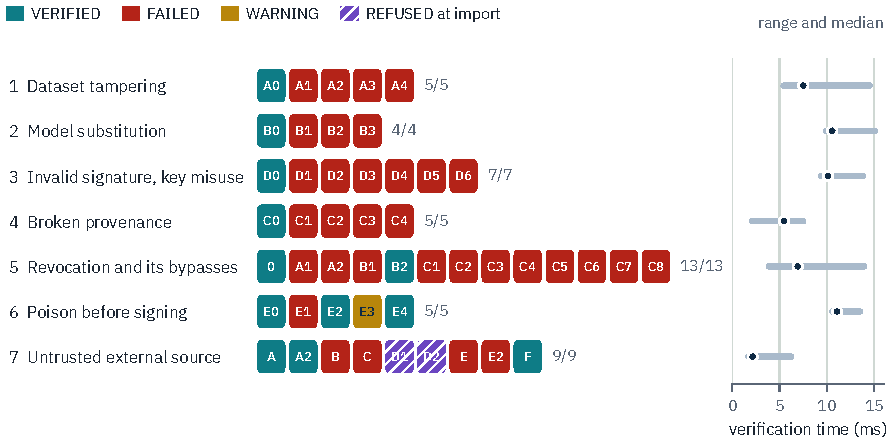
\includegraphics[width=\textwidth]{figures/fig_outcomes.pdf}
\caption{The 48 variants, one tile each, and the verification time of each experiment. The tiles of
experiments 5 and 7 omit the prefixes E5 and E7 of their identifiers. A \st{VERIFIED} tile is either an
untouched control or a case where \st{VERIFIED} was the predicted status, as for E2, E4 and E7-F
(Section~\ref{sec:boundary}).}
\label{fig:outcomes}
\end{figure}

\begin{table}[H]
\caption{The seven experiments: 48 variants, all with the predicted status.}
\label{tab:suite}
\tablefont
\begin{tabularx}{\textwidth}{P{0.55cm}P{4.3cm}rLP{2.35cm}}
\toprule
\headrow\hd{} & \hd{Experiment (scenario)} & \hd{Variants} & \hd{Outcome} & \hd{Checks that fired} \\
\midrule
1 & Dataset tampering (A) & 5 & control \cVER; 4 \cFAIL & V1, V2, V6 \\
2 & Model substitution (B) & 4 & control \cVER; 3 \cFAIL & V1 \\
3 & Invalid signature, key misuse (D) & 7 & control \cVER; 6 \cFAIL & V3, V4, V6 \\
4 & Broken provenance (C) & 5 & control \cVER; 4 \cFAIL & V3, V5, V8 \\
5 & Revocation and its bypasses (F) & 13 & 2 \cVER\ as predicted; 11 \cFAIL, the gateway blocks & V3, V4, V6, V7 \\
6 & Poison before signing (E) & 5 & 3 \cVER\ (E0, E2, E4); 1 \cFAIL\ (E1); 1 \cWARN\ (E3) & V6, V9 \\
7 & Untrusted external source (G) & 9 & 3 \cVER; 4 \cFAIL; 2 \cREF\ at import & V1, V3, V4, V6 \\
\bottomrule
\end{tabularx}
\end{table}

Every manipulation made after signing was rejected, including the subtle ones:
\begin{itemize}
\item \textbf{On datasets:} flipping the labels of five rows, appending one row, or adding a single trailing
  space to one line of a signed file. The report names the changed lines (V1, V2).
\item \textbf{On models:} replacing the file, nudging one weight by $10^{-6}$, which leaves the test accuracy
  unchanged, or saving identical weights again in the pickle format (V1). Integrity is stricter than
  behaviour: a functionally identical model is still rejected.
\item \textbf{On provenance:} deleting a parent record, editing a parent link without signing again, or
  presenting a validly signed model with no dataset ancestry (V5, V3, V8). In variant C2 an insider modifies the
  dataset and signs it again \emph{with the real data-steward key}: the dataset alone verifies, and the model
  that descends from it fails at V5. A legitimate signature cannot rewrite history beneath existing
  descendants.
\item \textbf{On keys:} corrupting or replaying a signature, signing with an unknown or a revoked key, or
  using the data-steward key to sign a model (V3, V4).
\end{itemize}
Revoking an artifact or a key fails every descendant and blocks the deployment, while a dataset signed by
another role still verifies after the training key is revoked: the damage is limited to the revoked key.
Detection, measured as the verification time of the attacked artifact with its chain, took 1.7 to 15.1\,ms,
with a median of 7.5\,ms.

\subsection{Attacks on the trust itself}
Experiment~5 targets the mechanism that decides who is trusted. After a base model is revoked, eight bypasses
(C1 to C8) try to make its fine-tuned descendant verify again:
\begin{itemize}
\item \textbf{Editing the index} (deleting the row of the revoked artifact, C1; deleting the revoked key, C2;
  overwriting the cached status with \st{VERIFIED}, C3). These fail because the verifier never reads a cached
  status and treats a missing row as a revocation it cannot rule out.
\item \textbf{Clearing the \code{revoked} flag in SQLite} (C4). This was the documented limitation of version
  0.3. It now fails: the signed log still says revoked, and the disagreement raises an
  \code{INDEX\_TAMPERING} event (Figure~\ref{fig:bypass}).
\item \textbf{Inserting a rogue key} into the index with the training role and using it to sign a substituted
  model (C5). It fails because the key never entered the signed log.
\item \textbf{Attacking the log}: truncating it to drop the revocation (C6), editing the record in place (C7)
  and deleting the file (C8). All three fail closed: the replay no longer ends at the pinned head, or no longer
  verifies under the root key.
\end{itemize}
What remains trusted is what the threat model declared trusted: whoever holds the root key and can rewrite the
pin controls the trust decisions.

\begin{figure}[!htb]
\centering
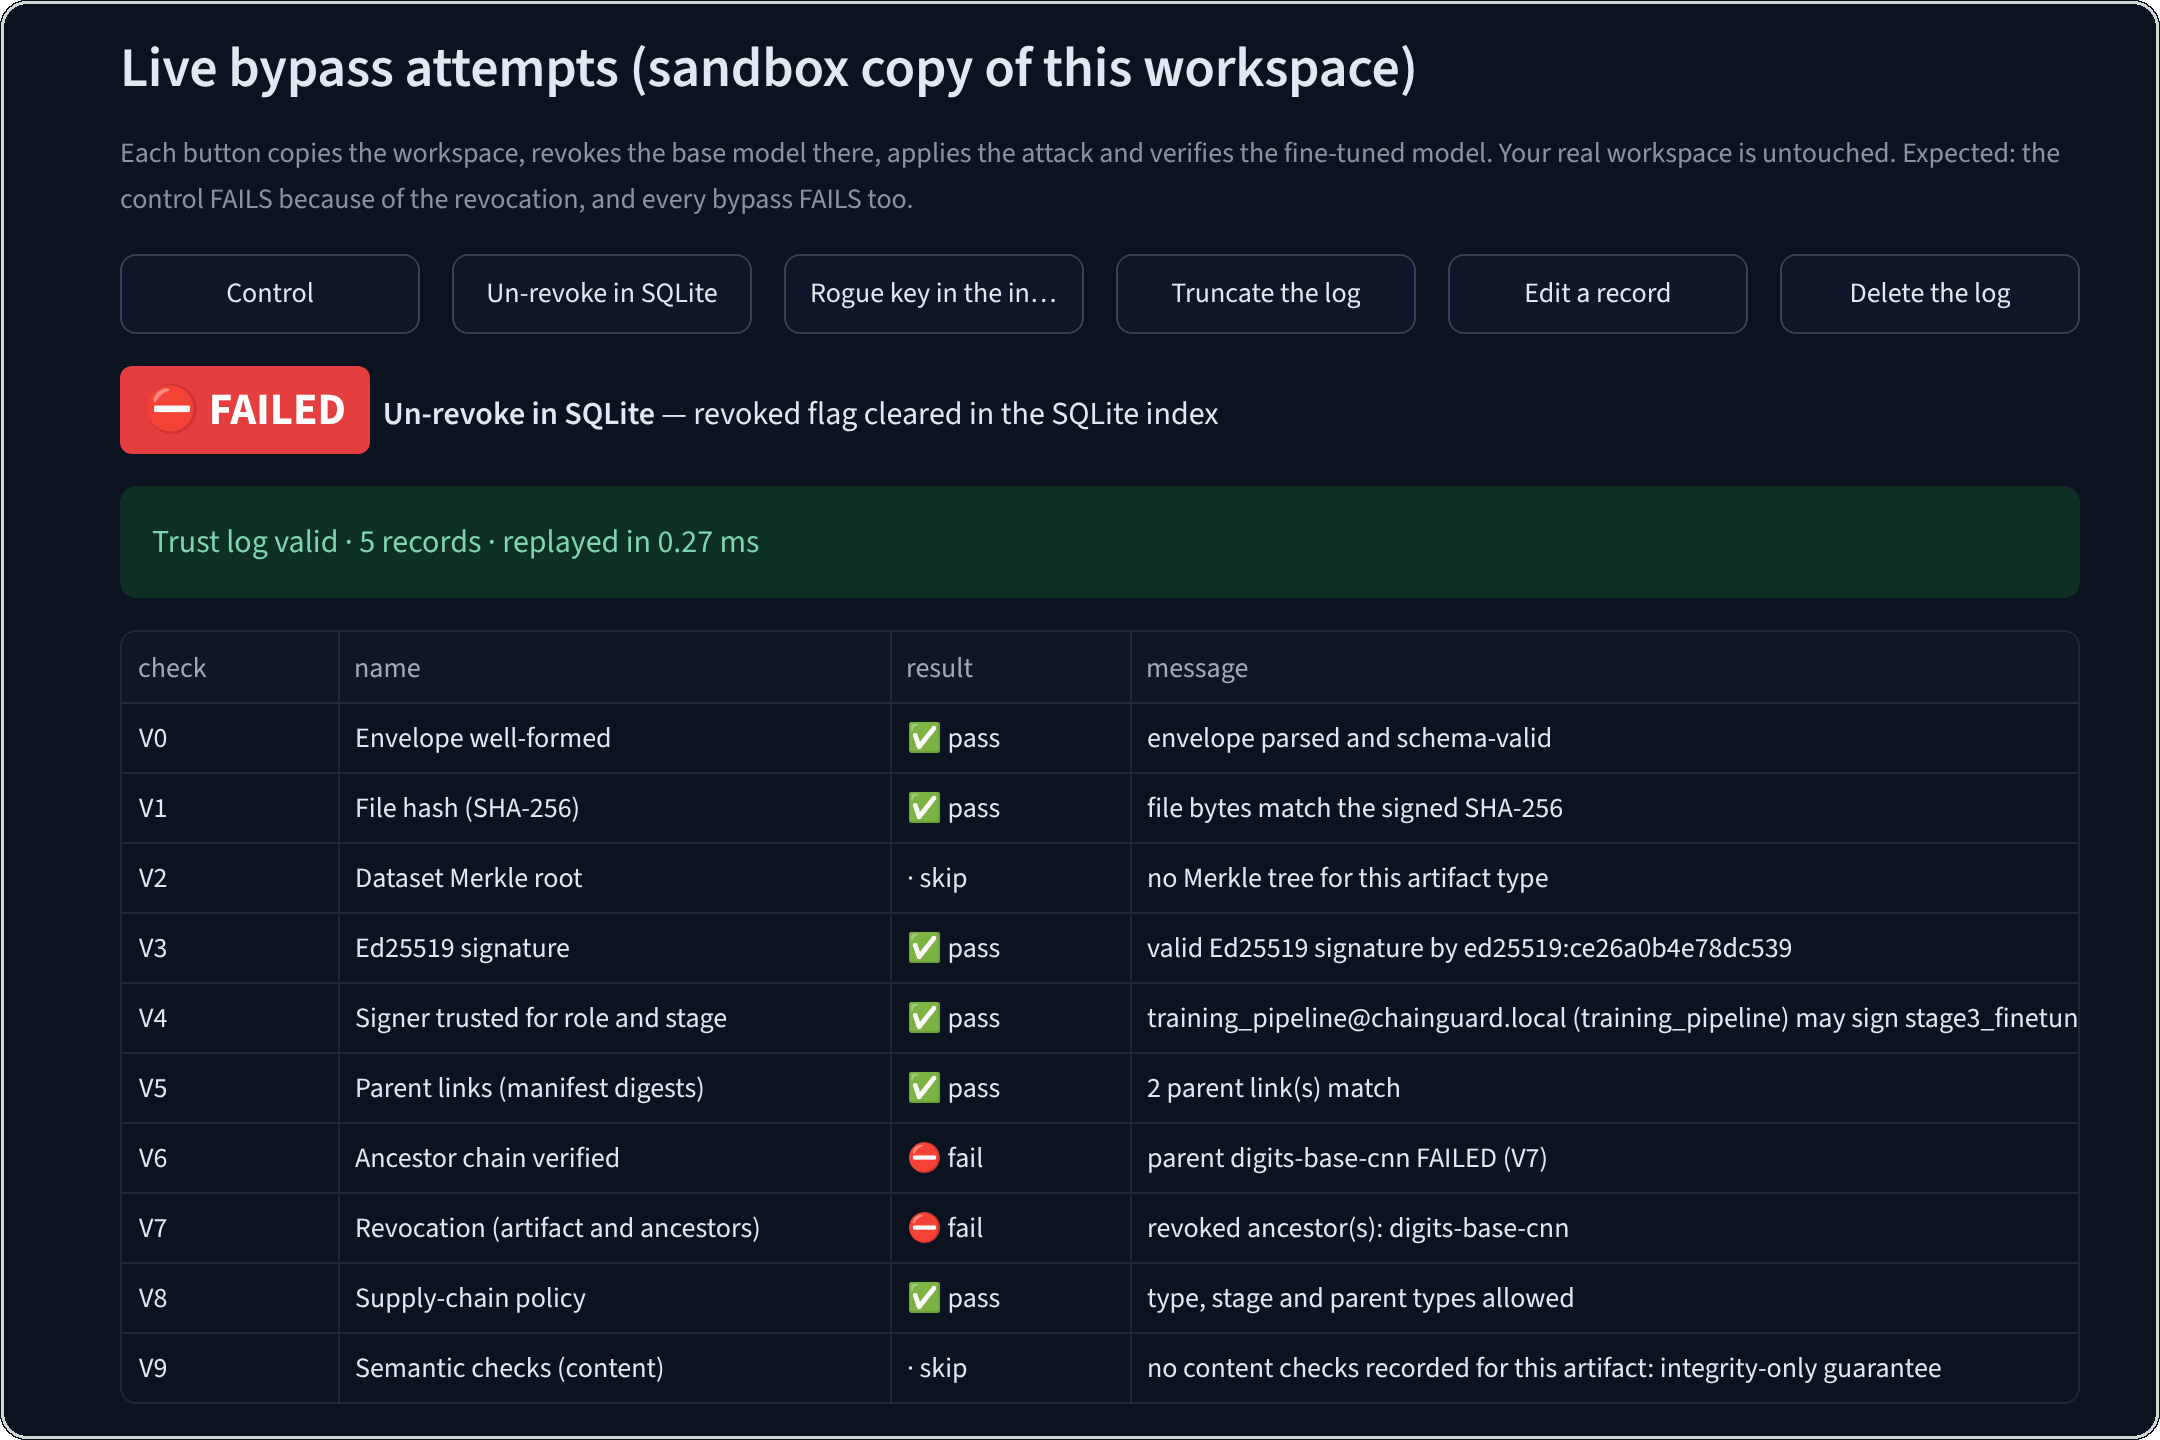
\includegraphics[width=0.72\textwidth]{figures/shot_trustlog.png}
\caption{Dashboard, trust log page: the bypass C4 replayed in a sandbox copy of the workspace (run of
10~November 2026). The revoked flag was cleared in the SQLite index; the fine-tuned model still fails at V6 and
V7 because the signed log is the authority.}
\label{fig:bypass}
\end{figure}

\subsection{Signed is not safe}
\label{sec:boundary}
Experiments 6 and 7 measure what the signature does not cover (Figure~\ref{fig:boundary}).

\begin{figure}[!htb]
\centering
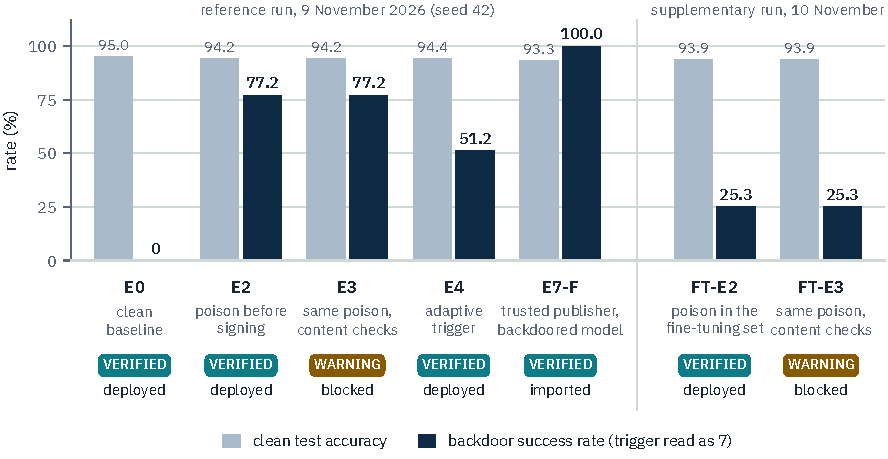
\includegraphics[width=\textwidth]{figures/fig_boundary.pdf}
\caption{Clean accuracy and backdoor success rate of the deployed or imported model, with its verification
status. Signed poison (E2), an adaptive trigger (E4) and the backdoored model of a trusted publisher (E7-F) pass
every cryptographic check. Content checks catch the trigger they know (E3, FT-E3).}
\label{fig:boundary}
\end{figure}

The clean pipeline (E0) deploys a model with a clean accuracy of 95.0\,\% and a backdoor success rate of
0\,\%. Poison injected into the signed dataset \emph{after} signing (E1) fails the chain at V6, as expected.
When the data steward signs a dataset that was poisoned \emph{before} attestation (E2), every check passes. The
fine-tuned model deploys as \st{VERIFIED} with a clean accuracy of 94.2\,\% (339 of the 360 held-out images),
within one point of the clean model, and a backdoor success rate of 77.2\,\% (250 of 324). Ordinary testing
would not reveal it.

With the content checks enabled before signing (E3), the known corner trigger and the shifted label
distribution are flagged. The dataset carries a signed flag, the model verifies with \st{WARNING} and the
gateway blocks it by default: heuristics work as evidence. An adaptive attacker who moves the trigger to a
pattern the checks do not know (E4, a bar on the left edge, 5\,\% of the rows) deploys as \st{VERIFIED} with a
backdoor success rate of 51.2\,\%.

Experiment 7 repeats the lesson at the boundary of the organisation. A backdoored model trained by a
\emph{trusted}, registered publisher (E7-F) imports as \st{VERIFIED} with a clean accuracy of 93.3\,\% and a
backdoor success rate of 100\,\%. The other variants are all rejected: the unknown publisher and the model
modified in transit are \st{FAILED}, the unsigned model and the manifest without its signature are \st{REFUSED}
at import, and the model of a publisher whose key was revoked is \st{FAILED}.

Fine-tuning on clean data weakens the backdoor without removing it: in E2 the base model has a backdoor success
rate of 99.1\,\%, which drops to 77.2\,\% after fine-tuning (99.4\,\% to 51.2\,\% in E4). Fine-tuning is not a
defence to rely on.

\begin{keybox}
\boxtitle{The result in one sentence.} A valid signature proves \emph{who} attested an artifact and \emph{that
nothing changed since}. It transfers trust to the signer and creates none.
\end{keybox}

\subsection{The four example tests of the brief}
The brief gives four example tests. Table~\ref{tab:brieftests} states where each one was run and what was
observed. The first one names the fine-tuning dataset, while experiment 6 poisons the training set of the base
model, so we ran it literally as a supplementary experiment on 10~November (FT-E2 and FT-E3, on the right of
Figure~\ref{fig:boundary}): 8\,\% of the 437 fine-tuning rows (35 rows) receive the corner trigger and the label
7 before the data steward signs them, and the base model is trained on clean data.

{\tablefont
\begin{xltabular}{\textwidth}{P{4.1cm}P{2.6cm}L}
\caption{The four example tests of the brief and what was observed.}\label{tab:brieftests}\\
\toprule
\headrow\hd{Example test of the brief} & \hd{Where} & \hd{Observed} \\
\midrule
\endfirsthead
\toprule
\headrow\hd{Example test of the brief} & \hd{Where} & \hd{Observed} \\
\midrule
\endhead
\bottomrule
\endfoot
Inject a backdoor into a fine-tuning dataset and verify detection failure or success & FT-E2, FT-E3 (and E2 to E4 for the training set) & Detection failure by cryptography: \cVER, deployed, clean accuracy 93.9\,\%, backdoor success 25.3\,\% (base model: 0\,\%). Detection success by the content checks: \cWARN, blocked \\
Substitute a signed model with a tampered version & Experiment 2 (B1 to B3) & Control \cVER. A different model, one weight changed by $10^{-6}$ and the same weights saved as pickle are all \cFAIL\ at V1; the gateway blocks \\
Verify the provenance of a model from an untrusted repository & Experiment 7 (nine variants) & Trusted publisher \cVER. Unknown publisher, model modified after signing and revoked publisher key \cFAIL. Unsigned model and stripped signature \cREF\ at import \\
Measure the attestation overhead on training and inference & Pipeline and inference benchmarks & Attestation 10.7\,ms against 1,288\,ms of training (0.83\,\%). One prediction: 0.084\,ms before and 0.085\,ms after the verified deployment \\
\end{xltabular}}

The backdoor of FT-E2 is weaker than that of E2 (25.3\,\% against 77.2\,\%) because eight epochs of fine-tuning
on 35 poisoned rows teach the model less than fifteen epochs of training on 80. The boundary is the same
wherever the poison enters before signing.

\subsection{Robustness to the random seed}
\label{sec:seeds}
The reference run uses one seed. The seed decides the split of the data, the rows that are poisoned, the
initial weights and the order of the mini-batches, so a single run could be a lucky or an unlucky draw. As a
second supplementary experiment on 10~November, we repeated the four pipeline variants of experiment 6 for ten
other seeds, 0 to 9 (Figure~\ref{fig:seeds}).

\begin{figure}[!htb]
\centering
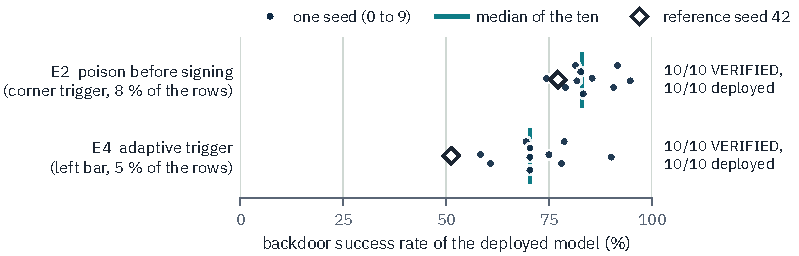
\includegraphics[width=\textwidth]{figures/fig_seeds.pdf}
\caption{Backdoor success rate of the deployed model for ten other seeds. The status never changes. The
reference seed gives the second weakest backdoor of the eleven runs for E2 and the weakest for E4.}
\label{fig:seeds}
\end{figure}

The verification status did not change once in the 40 runs:
\begin{itemize}
\item \textbf{E0, clean:} ten times \st{VERIFIED} and deployed; no content check raised a false alarm; clean
  accuracy 95.8 to 98.6\,\% (median 97.2\,\%); backdoor success rate 0\,\%.
\item \textbf{E2, poison before signing:} ten times \st{VERIFIED} and deployed; backdoor success rate 74.4 to
  94.8\,\% (median 83.0\,\%); clean accuracy 95.8 to 98.3\,\%.
\item \textbf{E3, same poison with content checks:} ten times \st{WARNING} and blocked.
\item \textbf{E4, adaptive trigger:} ten times \st{VERIFIED} and deployed; backdoor success rate 58.3 to
  90.1\,\% (median 70.4\,\%).
\end{itemize}
The run with the seed 42 reproduced the reference results exactly. The figures quoted in this report (77.2\,\%
and 51.2\,\%) are therefore at the low end of what the attack achieves, not a favourable draw.

\subsection{Cost}
\label{sec:cost}
Figure~\ref{fig:cost} gives the cost of each operation and Figure~\ref{fig:scaling} shows how it grows with
the size of what is attested.

\begin{figure}[!htb]
\centering
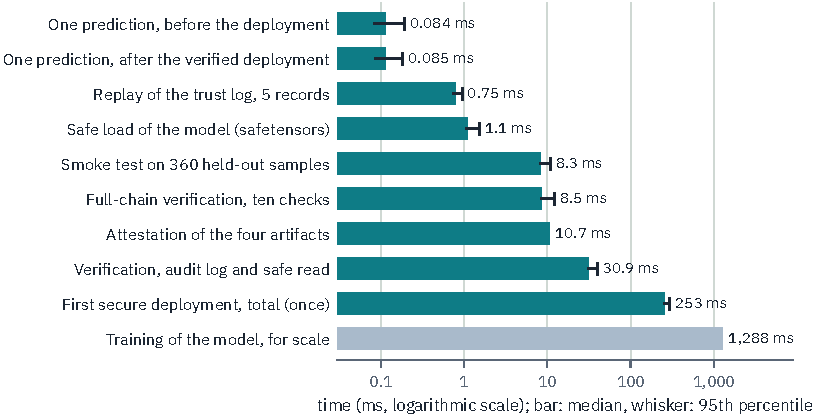
\includegraphics[width=\textwidth]{figures/fig_cost.pdf}
\caption{What attestation costs in the reference environment. Verification happens at deployment, so a
prediction costs the same before and after.}
\label{fig:cost}
\end{figure}

\textbf{Training.} Attesting the four artifacts of the pipeline took 10.7\,ms against 1,288\,ms of training,
or 0.83\,\%. The share depends on the workload and should shrink for larger models, because attestation grows
with the bytes of the artifacts while training grows with the computation.

\textbf{Verification.} A full-chain verification of the fine-tuned model with its three ancestors takes
8.5\,ms (median of 200 runs; 95th percentile 12.2\,ms). Replaying the five-record trust log accounts for
0.16\,ms of it; a first replay, in which every signature is verified, takes 0.75\,ms.

\textbf{Deployment.} The first secure deployment costs 253\,ms, once. The chain verification with its audit
writes and the safe read take 31\,ms, the safetensors load 1.1\,ms and the smoke test 8.3\,ms. The remaining
210\,ms or so go to signing and registering the deployment record, which verifies the chain a second time, and
to event and metric writes.

\textbf{Inference.} A prediction costs 0.084\,ms before and 0.085\,ms after the verified deployment
(medians of 1,000 runs each). Verification is not on the inference path.

\textbf{Storage.} A signed manifest is 1.4 to 3.1\,KB per artifact. The side file that holds the row hashes of
a dataset grows with the number of rows (30 and 68\,KB here).

\begin{figure}[!htb]
\centering
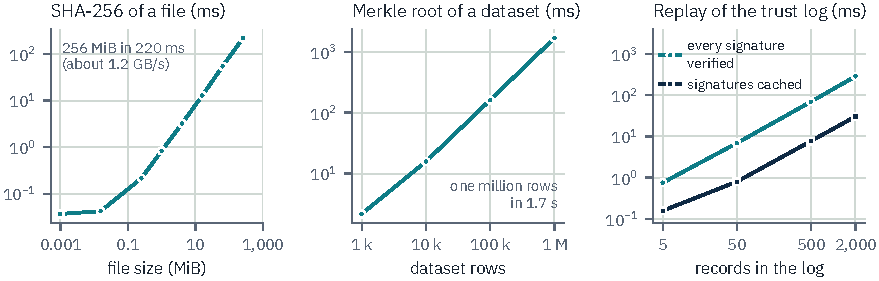
\includegraphics[width=\textwidth]{figures/fig_scaling.pdf}
\caption{How the cost grows. Hashing is linear in the size of the file and dominates for large artifacts;
signing and verifying a signature do not depend on the size (0.04\,ms and 0.12 to 0.14\,ms). Both axes are
logarithmic.}
\label{fig:scaling}
\end{figure}

\textbf{Scaling.} SHA-256 runs at about 1.2\,GB/s, so a model of 256\,MiB hashes in 220\,ms. The Merkle root of
a dataset of one million rows takes 1.7\,s. Replaying the trust log costs about 0.14\,ms per record when every
signature is verified (0.8, 6.9, 69 and 288\,ms for 5, 50, 500 and 2,000 records) and about 15 microseconds
per record with cached signatures. With thousands of records, one would checkpoint a signed snapshot of the
state instead of replaying from the first record.

\subsection{Tests and reproducibility}
\textbf{Automated tests.} 168 tests pass in 36\,s in the reference environment, with none failed and none
skipped: unit tests of hashing, canonical serialisation, signing, manifests, Merkle trees, the policy, the
content checks and the trust log; integration tests of registration and verification, the pipeline, the
revocation experiment, external models, the interoperability export, the API and the scenarios. The suite
grew with the system: 113 tests on 5~October, 143 on 16~October, 168 on 9~November.

\textbf{Continuous integration.} Both workflows passed on the first execution on GitHub (9~November) and on
every push since, on Python 3.11, a different version from the reference environment.

\textbf{Regeneration.} \code{python -m attacks.run\_all} regenerates every table of this section,
\code{python -m scripts.benchmark} and its companions every cost figure, and
\code{report/figures/make\_figures.py} every chart of this report from the result files
(Appendix~\ref{app:repro}).

\textbf{Verification by the reader.} The website serves the signed model of experiment E2, its signed manifest
and the public key. The page checks the file hash (V1) and the Ed25519 signature (V3) in the reader's browser
and runs the network in JavaScript: 339 of 360 clean images correct and 250 of 324 triggered images read as 7,
the figures of E2. Against PyTorch on all 684 inputs, the JavaScript network gave no different prediction.

\subsection{Threats to validity}
\begin{itemize}
\item \textbf{The attack suite is written by the defenders.} It shows that the checks behave as designed
  against the manipulations we thought of, not that no other manipulation exists.
\item \textbf{The model is small.} An 8 by 8 digit classifier shows how large the gap is on a small model, not
  that it has that size for a language model, where poisoning is cheaper \cite{souly2025}.
\item \textbf{The content checks are simple heuristics}, tuned by a defender who knows the trigger. E4 shows
  the cost of that assumption. Stronger detectors would raise the bar and, as adaptive attacks show, not close
  the gap.
\item \textbf{Timings come from one environment.} They were not measured again on team hardware, and shared
  CI runners are not a stable timing environment.
\item \textbf{One trigger family and one dataset.} The seed experiment varies the split, the poisoned rows
  and the initialisation, not the trigger family or the task.
\end{itemize}
None of this touches the central result, which holds by construction: a signature covers bytes, not behaviour.
